% -*- latex -*-

\chapter{Execution Environment}
\label{chap:ExecutionEnvironment}

\index{execution~environment|(}
\index{environment!execution|(}

The execution environment is exposed to developers that write worklets for
different visualization algorithms. In addition to providing all the
mechanisms for building the worklet object itself, the execution
environment contains supporting code that can be useful to the
implementations of visualization algorithms.

The data structures in the execution environment provide information and
operations for a single element. This is in contrast to the control
environment, where data structures are built on arrays providing
information for large collections of data. These respective data structures
reflect the nature of the two environments. The control environment manages
the stores of data whereas the execution environment performs large
parallel processing through fine operations.

\section{Working with Topology}
\label{sec:ExecutionEnvironment:WorkingWithTopology}

In the control environment, data is defined in mesh structures that
comprise a set of finite cells. (See Section~\ref{sec:DataSets:CellSets}
starting on page~\pageref{sec:DataSets:CellSets} for information on
defining cell sets in the control environment.) When worklets that operate
on cells are scheduled, these grid structures are broken into their
independent cells, and that data is handed to the worklet. Thus, cell-based
operations in the execution environment exclusively operate on independent
cells.

Unlike some other libraries such as VTK, VTK-m does not have a cell class
that holds all the information pertaining to a cell of a particular type.
Instead, VTK-m provides tags or identifiers defining the cell shape, and
companion data like coordinate and field information are held in separate
structures. This organization is designed so a worklet may specify exactly
what information it needs, and only that information will be loaded.

\subsection{Cell Shape Tags and Ids}
\label{sec:CellShapeTagsIds}

\index{shape|(}
\index{cell~shape|(}
\index{tag!cell~shape|(}
\index{tag!shape|(}

Cell shapes can be specified with either a tag (defined with a struct with
a name like \textidentifier{CellShapeTag*}) or an enumerated identifier
(defined with a constant number with a name like
\textidentifier{CELL\_SHAPE\_*}). These shape tags and identifiers are
defined in \vtkmheader{vtkm}{CellShape.h} and declared in the \vtkm{}
namespace (because they can be used in either the control or the execution
environment). Figure~\ref{fig:CellShapes} gives both the identifier and the
tag names.

\begin{figure}
  \centering
  \small
  \begin{tabular}{@{}c@{~}c@{~}c@{}}
    \raisebox{-0.5\height}{
\includegraphics{images/CellConnectionsVertex}} &
    \raisebox{-0.5\height}{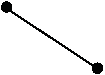
\includegraphics{images/CellConnectionsLine}} &
    \raisebox{-0.5\height}{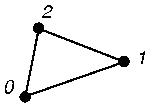
\includegraphics{images/CellConnectionsTriangle}} \\
    \vtkm{CELL\_SHAPE\_VERTEX} &
    \vtkm{CELL\_SHAPE\_LINE} &
    \vtkm{CELL\_SHAPE\_TRIANGLE} \\
    \vtkm{CellShapeTagVertex} \index{vertex} &
    \vtkm{CellShapeTagLine} \index{line} &
    \vtkm{CellShapeTagTriangle} \index{triangle} \\[2ex]
    \raisebox{-0.5\height}{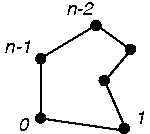
\includegraphics{images/CellConnectionsPolygon}} &
    \raisebox{-0.5\height}{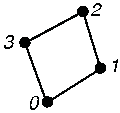
\includegraphics{images/CellConnectionsQuadrilateral}} &
    \raisebox{-0.5\height}{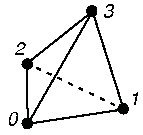
\includegraphics{images/CellConnectionsTetrahedron}} \\
    \vtkm{CELL\_SHAPE\_POLYGON} &
    \vtkm{CELL\_SHAPE\_QUAD} &
    \vtkm{CELL\_SHAPE\_TETRA} \\
    \vtkm{CellShapeTagPolygon} \index{polygon} &
    \vtkm{CellShapeTagQuad} \index{quadrilateral} &
    \vtkm{CellShapeTagTetra} \index{tetrahedron} \\[2ex]
    \raisebox{-0.5\height}{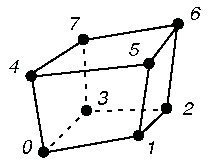
\includegraphics{images/CellConnectionsHexahedron}} &
    \raisebox{-0.5\height}{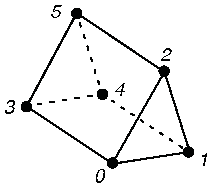
\includegraphics{images/CellConnectionsWedge}} &
    \raisebox{-0.5\height}{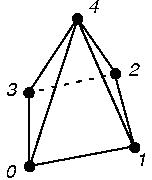
\includegraphics{images/CellConnectionsPyramid}} \\
    \vtkm{CELL\_SHAPE\_HEXAHEDRON} &
    \vtkm{CELL\_SHAPE\_WEDGE} &
    \vtkm{CELL\_SHAPE\_PYRAMID} \\
    \vtkm{CellShapeTagHexahedron} \index{hexahedron} &
    \vtkm{CellShapeTagWedge} \index{wedge} &
    \vtkm{CellShapeTagPyramid} \index{pyramid}
  \end{tabular}
  \caption{Basic Cell Shapes}
  \label{fig:CellShapes}
\end{figure}

In addition to the basic cell shapes, there is a special ``empty'' cell
with the identifier \vtkm{CELL\_SHAPE\_EMPTY} and tag
\vtkm{CellShapeTagEmpty}. This type of cell has no points, edges, or faces
and can be thought of as a placeholder for a null or void cell.

There is also a special cell shape ``tag'' named \vtkm{CellShapeTagGeneric}
that is used when the actual cell shape is not known at compile time.
\textidentifier{CellShapeTagGeneric} actually has a member variable named
\textcode{Id} that stores the identifier for the cell shape. There is no
equivalent identifier for a generic cell; cell shape identifiers can be
placed in a \vtkm{IdComponent} at runtime.

When using cell shapes in templated classes and functions, you can use the
\vtkmmacro{VTKM\_IS\_CELL\_SHAPE\_TAG} to ensure a type is a valid cell
shape tag. This macro takes one argument and will produce a compile error
if the argument is not a cell shape tag type.

\subsubsection{Converting Between Tags and Identifiers}

Every cell shape tag has a member variable named \textcode{Id} that
contains the identifier for the cell shape. This provides a convenient
mechanism for converting a cell shape tag to an identifier. Most cell shape
tags have their \textcode{Id} member as a compile-time constant, but
\textidentifier{CellShapeTagGeneric} is set at run time.

\vtkmheader{vtkm}{CellShape.h} also declares a templated class named
\vtkm{CellShapeIdToTag} that converts a cell shape identifier to a cell
shape tag. \textidentifier{CellShapeIdToTag} as a single template argument
that is the identifier. Inside the class is a type named \textcode{Tag}
that is the type of the correct tag.

\vtkmlisting{Using \textidentifier{CellShapeIdToTag}.}{CellShapeIdToTag.cxx}

However, \textidentifier{CellShapeIdToTag} is only viable if the identifier
can be resolved at compile time. In the case where a cell identifier is
stored in a variable or an array or the code is using a
\textidentifier{CellShapeTagGeneric}, the correct cell shape is not known
at run time. In this case, \vtkmmacro{vtkmGenericCellShapeMacro} can be
used to check all possible conditions. This macro is embedded in a switch
statement where the condition is the cell shape identifier.
\vtkmmacro{vtkmGenericCellShapeMacro} has a single argument, which is an
expression to be executed. Before the expression is executed, a type named
\textcode{CellShapeTag} is defined as the type of the appropriate cell
shape tag. Often this method is used to implement the condition for a
\textidentifier{CellShapeTagGeneric} in a function overloaded for cell
types. A demonstration of \vtkmmacro{vtkmGenericCellShapeMacro} is given in
Example~\ref{ex:GenericCellNormal}.

\index{tag!shape|)}
\index{tag!cell~shape|)}

\subsubsection{Cell Traits}

\index{cell~traits|(}

The \vtkmheader{vtkm}{CellTraits.h} header file contains a traits class
named \vtkm{CellTraits} that provides information about a cell. Each
specialization of \textidentifier{CellTraits} contains the following
members.

\begin{description}
\item[\textcode{TOPOLOGICAL\_DIMENSIONS}] Defines the topological
  dimensions of the cell type. This is 3 for polyhedra, 2 for polygons, 1
  for lines, and 0 for points.
\item[\textcode{TopologicalDimensionsTag}] A type set to either
  \vtkm{CellTopologicalDimensionsTag}\textcode{<3>},
  \textidentifier{CellTopologicalDimensionsTag}\textcode{<2>},
  \textidentifier{CellTopologicalDimensionsTag}\textcode{<1>}, or
  \textidentifier{CellTopologicalDimensionsTag}\textcode{<0>}. The number
  is consistent with \textcode{TOPOLOGICAL\_DIMENSIONS}. This tag is
  provided for convenience when specializing functions.
\item[\textcode{IsSizeFixed}] Set to either \vtkm{CellTraitsTagSizeFixed}
  for cell types with a fixed number of points (for example, triangle) or
  \vtkm{CellTraitsTagSizeVariable} for cell types with a variable number of
  points (for example, polygon).
\item[\textcode{NUM\_POINTS}] A \vtkm{IdComponent} set to the number of
  points in the cell. This member is only defined when there is a constant
  number of points (i.e. \textcode{IsSizeFixed} is set to
  \vtkm{CellTraitsTagSizeFixed}).
\end{description}

\vtkmlisting[ex:GenericCellNormal]{Using \textidentifier{CellTraits} to implement a polygon normal estimator.}{GenericCellNormal.cxx}

\index{cell~traits|)}

\index{cell~shape|)}
\index{shape|)}

\subsection{Parametric and World Coordinates}

\index{parametric~coordinates|(}
\index{world~coordinates|(}
\index{cell!parametric~coordinates|(}
\index{cell!world~coordinates|(}

Each cell type supports a one-to-one mapping between a set of parametric
coordinates in the unit cube (or some subset of it) and the points in 3D
space that are the locus contained in the cell. Parametric coordinates are
useful because certain features of the cell, such as vertex location and
center, are at a consistent location in parametric space irrespective of
the location and distortion of the cell in world space. Also, many field
operations are much easier with parametric coordinates.

The \vtkmheader{vtkm/exec}{ParametricCoordinates.h} header file contains the
following functions for working with parametric coordinates.

\begin{description}
\item[\vtkmexec{ParametricCoordinatesCenter}] Returns the parametric
  coordinates for the center of a given shape. It takes 4 arguments: the
  number of points in the cell, a \vtkm{Vec} of size 3 to store the
  results, a shape tag, and a worklet object (for raising errors). A second
  form of this method takes 3 arguments and returns the result as a
  \vtkm{Vec}\textcode{<}\vtkm{FloatDefault}\textcode{,3>} instead of
  passing it as a parameter.
\item[\vtkmexec{ParametricCoordinatesPoint}] Returns the parametric
  coordinates for a given point of a given shape. It takes 5 arguments: the
  number of points in the cell, the index of the point to query, a
  \vtkm{Vec} of size 3 to store the results, a shape tag, and a worklet
  object (for raising errors). A second form of this method takes 3
  arguments and returns the result as a
  \vtkm{Vec}\textcode{<}\vtkm{FloatDefault}\textcode{,3>} instead of
  passing it as a parameter.
\item[\vtkmexec{ParametricCoordinatesToWorldCoordinates}] Given a vector of
  point coordinates (usually given by a \sigtag{FieldPointIn} worklet
  argument), a \vtkm{Vec} of size 3 containing parametric coordinates, a
  shape tag, and a worklet object (for raising errors), returns the world
  coordinates.
\item[\vtkmexec{WorldCoordinatesToParametricCoordinates}] Given a vector of
  point coordinates (usually given by a \sigtag{FieldPointIn} worklet
  argument), a \vtkm{Vec} of size 3 containing world coordinates, a shape
  tag, and a worklet object (for raising errors), returns the parametric
  coordinates. This function can be slow for cell types with nonlinear
  interpolation (which is anything that is not a simplex).
\end{description}

\index{cell!world~coordinates|)}
\index{cell!parametric~coordinates|)}
\index{world~coordinates|)}
\index{parametric~coordinates|)}

\subsection{Interpolation}

\index{cell!interpolation|(}
\index{interpolation|(}

The shape of every cell is defined by the connections of some finite set of
points. Field values defined on those points can be interpolated to any
point within the cell to estimate a continuous field.

The \vtkmheader{vtkm/exec}{CellInterpolate.h} header contains the function
\vtkmexec{CellInterpolate} that takes a vector of point field values
(usually given by a \sigtag{FieldPointIn} worklet argument), a \vtkm{Vec}
of size 3 containing parametric coordinates, a shape tag, and a worklet
object (for raising errors). It returns the field interpolated to the
location represented by the given parametric coordinates.

\vtkmlisting{Interpolating field values to a cell's center.}{CellCenters.cxx}

\index{interpolation|)}
\index{cell!interpolation|)}

\subsection{Derivatives}

\index{cell!derivative|(}
\index{cell!gradient|(}
\index{derivative|(}
\index{gradient|(}

Since interpolations provide a continuous field function over a cell, it is
reasonable to consider the derivative of this function. The
\vtkmheader{vtkm/exec}{CellDerivative.h} header contains the function
\vtkmexec{CellDerivative} that takes a vector of scalar point field values
(usually given by a \sigtag{FieldPointIn} worklet argument), a \vtkm{Vec}
of size 3 containing parametric coordinates, a shape tag, and a worklet
object (for raising errors). It returns the field derivative at the
location represented by the given parametric coordinates. The derivative is
return in a \vtkm{Vec} of size 3 corresponding to the partial derivatives
in the $x$, $y$, and $z$ directions. This derivative is equivalent to the
gradient of the field.

\vtkmlisting{Computing the derivative of the field at cell centers.}{CellDerivatives.cxx}

\index{gradient|)}
\index{derivative|)}
\index{cell!gradient|)}
\index{cell!derivative|)}

\index{environment!execution|)}
\index{execution~environment|)}
